%! Mode:: "TeX:UTF-8"
%! TEX program = xelatex
\PassOptionsToPackage{quiet}{xeCJK}
\documentclass[withoutpreface,bwprint]{cumcmthesis}
\usepackage{etoolbox}
\BeforeBeginEnvironment{tabular}{\zihao{-5}}
\usepackage[numbers,sort&compress]{natbib}  % 文献管理宏包
\usepackage[framemethod=TikZ]{mdframed}  % 框架宏包
\usepackage{url}  % 网页链接宏包
\usepackage{subcaption}  % 子图宏包
\usepackage{graphicx}
\usepackage{booktabs,colortbl}
\usepackage{xcolor}
\usepackage{xcolor}
\usepackage{tikz}
\usepackage{array}
\newcommand{\headcol}[1]{\textbf{#1}} % 假设你想要加粗表格的表头列
\tikzstyle{point}=[coordinate,on grid,]  
\usetikzlibrary{arrows,shapes,chains}
\usetikzlibrary{positioning, shapes.geometric,arrows,chains}
\usetikzlibrary{shapes.geometric, arrows,chains} 
\usepackage{indentfirst}
\usepackage{amsmath}
\newcolumntype{C}{>{\centering\arraybackslash}X}
\newcolumntype{R}{>{\raggedleft\arraybackslash}X}
\newcolumntype{L}{>{\raggedright\arraybackslash}X}
\usepackage{tikz}
\usepackage{listings}
\usepackage{xcolor} % 可选,用于代码高亮
\usetikzlibrary{arrows.meta} % 加载箭头元库


\title{基于驾驶员行为分析的交通信号灯黄灯时长优化研究\\ \small{顾晨曦 Chenxi.Gu22@student.xjtlu.edu.cn}\\\small{范訸然 Heran.Fan22@student.xjtlu.edu.cn}\\\small{须一菲 Yifei.Xu2202@}student.xjtlu.edu.cn\\}  % 论文标题
\tihao{}  % 题号
\baominghao{}  % 报名号
\schoolname{}  % 学校
\membera{}  % 队员a
\memberb{}  % 队员b
\memberc{}  % 队员c
\supervisor{}  % 指导老师
\yearinput{}
\monthinput{}
\dayinput{}

%%%%%%%%%%%%%%%%%%%%%%%%%%%%%%%%%%%%%%%%%%%%%%%%%%%%%%%%%%%%%
%% 正文
\begin{document}
\maketitle
\begin{abstract}
	本模型核心在于对黄灯相位周期内车辆行进过程的分段研究,并对合理黄灯时长的影响因子的作用进行具体探究,针对现行黄灯时长提出合理建议,针对问题一,我们采用控制变量方式,基于理想条件和现实参数分别建立匀速前进的模型一和变速的模型二,并对不同初速度机动车辆的不同情况进行分类。针对问题二,我们带入基于现实情况的各项参数数值,对计算得出的具体黄灯时长进行分析与现行较为普遍的$3-4s$进行对比分析。
	
\textbf{对于问题一,}首先,我们构建了基于理想化交通环境的黄灯时长数学模型;其次,我们考虑了实际交通条件下的参数变化,如驾驶员反应时间、不同车型和道路条件,进一步建立了模型二;同时对不同初速度机动车辆的不同情况进行分类,分别探究初速度和绿灯变黄灯时距停止线距离对合理黄灯时长的具体影响。

\textbf{对于问题二,}利用控制变量法,分别探究有无黄灯倒计时,初速度大小,离停止线距离大小,行驶方向对于合理黄灯时长的影响,结果表明,在有黄灯倒计时,初速度更大,离停止线更远,直行情况下,为保证所有车辆都顺利通过交叉路口,应设置更久的黄灯时长来确保安全性。

\textbf{对于问题三,}为评估模型下机动车通过交叉路口的效率,本研究计算了车辆通过本侧停止线与对侧停止线所需时间的相关系数。通过两两间相关系数的计算,我们能够量化车辆通过交叉口的相互依赖性。在此基础上进一步绘制了热力图以直观展示不同车辆间的时间关联性,验证模型的可行性和优越性,并进一步分析模型潜在优势,提出改进方向。

结果表明,通过合理调整黄灯时长,可以显著提高车辆的通过率,减少交叉口内的交通事故。此外,我们还探讨了延长黄灯时长可能带来的潜在问题,如通行时间的不确定性增加和对交通流量的影响。
%本研究针对城市交通信号灯黄灯时长设置问题,采用数学建模和数据分析方法,对影响黄灯时长的关键因素进行了深入探讨。文章首先概述了黄灯在交通信号控制中的重要性及其在交通事故预防中的作用。通过对现有法规和驾驶员行为的分析,我们建立了考虑不同初始速度、行驶距离和反应时间等因素的数学模型,旨在优化黄灯时长设置,提高交叉口的通行效率和安全性。
%
%研究分为三个主要部分:首先,我们构建了基于理想化交通环境的黄灯时长数学模型;其次,我们考虑了实际交通条件下的参数变化,如驾驶员反应时间、不同车型和道路条件,进一步细化了模型;最后,我们将模型结果与现行标准进行比较,分析了模型的优势和局限性,并提出了优化建议。
%
%本研究的创新点在于综合考虑了多种影响因素,并通过实际数据验证了模型的有效性。结果表明,通过合理调整黄灯时长,可以显著提高车辆的通过率,减少交叉口内的交通事故。此外,我们还探讨了延长黄灯时长可能带来的潜在问题,如通行时间的不确定性增加和对交通流量的影响。

\keywords{边界建模\quad  左转相位 \quad Pearson 相关系数 \quad 二次多项式拟合}
\end{abstract}
%%%%%%%%%%%%%%%%%%%%%%%%%%%%%%%%%%%%%%%%%%%%%%%%%%%%%%%%%%%%% 

\tableofcontents  % 目录
\newpage

%%%%%%%%%%%%%%%%%%%%%%%%%%%%%%%%%%%%%%%%%%%%%%%%%%%%%%%%%%%%%  
\section{问题重述}
\subsection{问题背景}
红绿灯是一种交通管制设施,通过红、黄、绿三种颜色的灯光交替变换,来规定道路通行权,确保车辆和行人的安全通行。交叉口是红绿灯的最常见使用场景,是城市道路的关键节点,更是交通事故的频发地。据统计,黄灯时间内发生的交通事故约占整个信号交叉口交通事故的 50%以上。

为确保道路交通安全,我国已经出台多项强制性法规,明确规定了机动车在遇到黄灯信号时应遵循的行驶规则,以减少各类交通事故的发生。2004年发布的《中华人民共和国道路交通安全法实施条例》第三十八条规定:“黄灯亮时,已越过停止线的车辆可以继续通行”,《道路交通安全法》规定黄灯表示警示,并规定机动车遇路口时应减速通过“黄灯亮时已经越过停止线的车辆可以继续通过,还未越过停止线的车辆应停车。抢黄灯行为属于违反道路交通信号灯通行,对驾驶人处20元以上200元以下罚款,记6分。”

然而,现实生活中,往往存在着车辆已经预备进入交叉路口但尚未完全通过或汽车距离停止线过近即使以最大加速度刹车也无法停止,但信号灯即将或已经从绿灯变为黄灯情况。这种情况下汽车可能无法及时制动,从而造成交通事故。通过研究相关影响因素,制定更加合理的黄灯时长,使正行驶在路口或离路口太近而无法安全停下的车辆能安全通过路口,可以有效降低此类交通事故发生可能性。


\begin{tikzpicture}[
	% 定义粗箭头样式
	thick_arrow/.style={
		postaction={
			-Stealth, % 使用Stealth箭头样式
			draw,      % 绘制箭头
			thick      % 设置箭头为粗线条
		}
	}
	]
	
	% 画带粗箭头的直线

\end{tikzpicture}
\subsection{问题要求}
\begin{enumerate}
  \item \textcolor{black}{问题一:问题一为开放式问题,需要在未知情况下综合考虑初速度、行驶距离等各种与黄灯最优时长有关的直接、间接因素,模拟机动车在交通信号灯由绿转黄时汽车的行驶过程,分析归纳,建立合适的数学模型。}
  \item \textcolor{black}{问题二:在实际测算中,不同参数有相应取值范围,根据参数具体值我们可以确定黄灯的具体时长,以确保在不同的交通条件下驾驶员都能获得足够的反应时间来安全地停车或通过交叉口。综合考虑各个参数的具体值,模拟在不同路况下黄灯的合理时长。}
  \item \textcolor{black}{问题三:将模型运用到现实场景,将计算结果与现行标准进行比较,呈现模型优势与不足。基于此对比分析,提出针对性模型优化建议,以期提升模型的实用性和准确性。}
\end{enumerate}

%%%%%%%%%%%%%%%%%%%%%%%%%%%%%%%%%%%%%%%%%%%%%%%%%%%%%%%%%%%%% 

\section{问题分析}
%\subsection{数据预处理}
% \textcolor{black}{\normalsize 由于题目给定数表分散,单品名称,品类名称,损耗率分布在不同表格中,因此需要进行数表合并。且本题需处理数据数量庞大,因此为防止海量的原始数据中存在着不完整(有缺失值)、不一致、有异常的数据,影响后题结果,需要对数据进行清洗。}
% 
% \textcolor{black}{\normalsize 数表合并:运用excel表格里的vlookup,sumif和sumifs函数,将附件1中品类的种类对应至其他表格中,方便题目所给问题的分析} 
% 
%  \textcolor{black}{​\normalsize 经过筛选,发现图表中没有空白值和缺失值,依据$3\sigma$原则,去除$>3\sigma$和$<3\sigma$的异常销量值,表中存在大量负值,及存在退货情况,由于退货会对应先前一笔购买账单,在此不讲退货情况单独计入,并将退货对应的销量负值替换为排除退货销量的销量均值$\mu$} 
\subsection{问题一的分析}
在理想化的交通模型中,车辆从信号灯绿转黄至完全通过路口速度不变,需要考虑从绿灯变黄灯起至汽车车身完全通过路口,全程保持初始速度$v_0$的情况。
%\begin{figure}
%	\centering
%	\begin{tikzpicture} [>=latex, scale = 0.8]
%		% 画半圆,中心在(0,0),半径为2cm
%		\draw (-3,2) arc (270:360:1cm);
%		\draw (-2,-3) arc (0:90:1cm);
%		\draw (2,3) arc (180:270:1cm);
%		\draw (3,-2) arc (90:180:1cm);
%		% 可以添加一些辅助线或标记
%		\fill (0,0) circle (2pt); % 标记圆心
%		\draw (3,2) -- (7,2); 
%		\draw (3,-2) -- (7,-2); 
%		\draw (-3,2) -- (-7,2); 
%		\draw (-3,-2) -- (-7,-2); 
%		\draw (2,3) -- (2,7); 
%		\draw (2,-3) -- (2,-7); 
%		\draw (-2,-3) -- (-2,-7); 
%		\draw (-2,3) -- (-2,7); 
%		\draw (-1,0) -- (1,0); % x轴
%		\draw (0,-1) -- (0,1); % y轴
%		\draw (0,3) -- (0,7); 
%		\draw (0,-3) -- (0,-7); 
%		\draw (3,0) -- (7,0); 
%		\draw (-3,0) -- (-7,0); 
%		\draw[line width=1.5pt, ->] (1,-4) -- (1,-2.2);
%		\draw[line width=1.5pt] (1.5,-4) -- (1.5,-2.7);
%		\draw[line width=1.5pt, ->] (1.5,-2.7) -- (1.8,-2.2);
%		\draw[line width=1.5pt] (1,-2.2) -- (1,-2);
%	\end{tikzpicture}
%\caption{双向三车道十字路口示意图}
%\end{figure}

依据《中华人民共和国道路交通安全法》第四十四条规定:机动车通过交叉路口,应当按照交通信号灯、交通标志、交通标线或者交通警察的指挥通过;通过没有交通信号灯、交通标志、交通标线或者交通警察指挥的交叉路口时,应当减速慢行,且在通过路口时速度应小于30$km/h$。因此需要进一步考虑当绿灯变黄灯时刻,司机经过反应踏减速踏板,进行减速过程下黄灯设置的不同时长。由于机动车的不同初速度,存在需要减速的不同距离,依据是否在停止线前将速度减至规定30$km/h$,将模型分类。

%%%%%%%%%%%%%%%%%%%%%%%%%%%%%%%%%%%%%%%%%%%%%%%%%%%%%%%%%%%%% 
\subsection{问题二的分析}
问题二立足于问题一模型,对过往文献中记录的驾驶员反应时间,不同道路上不同限速等车辆行为和路况数据进行了研究综述。在此基础上,我们特别关注了交通信号灯变换期间,左转车辆与直行车辆在路口所需行驶距离的差异性,以及公交车与轿车等不同车型因其不同车身长度而对路口通行效率所产生的影响。

此外,考虑到黄灯闪烁时是否有装配倒计时装置是影响整个交通流程总时长的关键因素,本研究进一步探讨了这一因素对合理设置黄灯时长的具体影响。

为了系统地研究这些变量之间的关系,需采用了控制变量法,对模型一和模型二在不同条件下的适用性进行对比分析,考察某一变量变化对黄灯时长设置的潜在影响。


\subsection{问题三的分析}
考虑到模型应用于实际场景时所面临的复杂可能性,将第二问得出的黄灯时长优化结果与现行的黄灯时长标准进行综合比较分析,在过程中进一步考虑此前未曾涉及的可能性。同时进行对比分析,分别计算在现行黄灯时长和模型模拟黄灯时长下末行车辆分别对与本侧停止线和对侧停止线通过的可能性,分析此指标优劣以及相关原因,进一步说明模型的潜在优越性。
\section{模型假设}
\subsection{基本假设}
\begin{enumerate}
	\item 本题仅探讨左转和直行车辆,假设右转车辆对其他车道车辆无影响。
	\item 假设所研究区域所有车辆遵守《中华人民共和国道路交通安全法》,在路口内不进行加速。
	\item 假设司机在看到绿灯变黄灯时反应和决策过程中汽车保持匀速前进。
	\item 假设分析对象前方没有车辆,即对象处于开阔的道路条件下,其他车辆对分析对象的速度无影响。
	\item 假设不存在侧方突然冲出的行人,非机动车等不确定因素。
	\item 假设模型中所涉及的函数都是随时间连续变化的,可微的函数。
\end{enumerate}
\subsection{模型一假设}
\begin{enumerate}
  \item 假设红绿灯在此种情况黄灯变红灯时无倒计时。
  \item 假设左转和直行车辆在看到绿灯变黄时均不减速。
\end{enumerate}

\section{符号说明}
\subsection{问题一符号说明}
%tab1
\begin{table}[htb!]
  \centering
  \small
  \begin{tabular}{p{60pt}<{\centering}|p{60pt}<{\centering}p{180pt}<{\raggedright}}
   \hline
   \rowcolor{gray!25} % 设置行颜色为25%的灰色
   \headcol \textbf{序号} & \textbf{符号} & \textbf{符号说明} \\
   \hline
    1 & $t_0$ & 驾驶员反应和决策时间(s) \\
    2 & $x_0$ & 驾驶员反应和决策时间内行驶距离(m) \\
    3 & $t_1$ & 车辆减速时间(s)\\
    4 & $t_2$ & 驾驶员做出决策至车头触碰停止线所经历的时间(s)\\
    5 & $L$ & 车身长度(m) \\
    6 & $H$ & 路口宽度(m) \\
    7 & $v_0$ & $t = 0$汽车初始速度(m/s) \\
    8 & $v_F$ & 法规规定的通过路口的标准速度($30m/s$)(m/s) \\
    9 & $a_1$ & $t = 0$在保证安全的情况下汽车减速最大制动力下的加速度(m/s) \\
    10 & $a_2$ & $t = 0$参考减速加速度(m/s) \\
    11 & $a_0$ & $t = 0$参考减速加速度(m/s) \\
    12 & $S$ & 绿灯变黄灯时距停止线距离(m) \\
%    6 & $r(t)$& 知谣不传谣者占学生比重\\
%    7 & $r_{0}$& $t=0$谣言免疫者占学生的比重\\
%    8 & $\lambda$ & 单位时间内每个信谣传谣者接触人数(人/$H$) \\
%    9 & $\mu$ & 单位时间内每个信谣传谣者转化为谣言免疫者人数(人/$H$)  \\
%    10 & $P=\dfrac{\lambda}{\mu}$& 谣言传播强度\\
	\hline
  \end{tabular}
%  \caption{问题一符号与说明}
  \label{symbol}
\end{table}

%\subsection{问题二补充符号说明}
%%tab1
%\begin{table}[htb!]
%	\centering
%	\small
%	\begin{tabular}{p{60pt}<{\centering}|p{60pt}<{\centering}p{180pt}<{\raggedright}}
%		\hline
%		\headcol 序号 & 符号 & 符号说明 \\
%		\hline
%		1 & $j(t)$ & 谣言判断者总学生比重 \\
%		2 & $w(t)$ & 真实信息传播者占总学生比重\\
%		3 & $a$ & 单位时间内谣言未知者转化为谣言判断者人数(人/$H$)\\
%		4 & $b$ &单位时间内谣言未知者转化为信谣传谣者人数(人/$H$) \\
%		5 & $c$ & 单位时间内谣言未知者转化为真实信息传播者人数(人/$H$) \\
%		6 & $d$& 单位时间内谣言未知者转化为谣言免疫者人数(人/$H$)\\
%		7 & $e$& 单位时间内谣言判断者转化为信谣传谣者人数(人/$H$)\\
%		8 & $f$ & 单位时间内谣言判断者转化为真实信息传播者人数(人/$H$)) \\
%		9 & $g$ & 单位时间内谣言判断者转化为谣言免疫者人数(人/$H$)  \\
%		10 & $l$ & 单位时间内信谣传谣者转化为谣言免疫者人数(人/$H$)  \\
%		\hline
%	\end{tabular}
%%	\caption{问题二符号与说明}
%	\label{symbol2}
%\end{table}



 \newpage
\section{模型的建立与问题的求解}
\subsection{问题一的求解}
\subsubsection{模型一的建立}
依据现实情况将驾驶员从反应到通过路口过程依据驾驶员反应时间分为三段,及驾驶员反应和决策时间内汽车行驶过程$x_0$,驾驶员采取行动至车头触碰停止线形式距离$x_1$,汽车在保证安全的情况下最大减速度为$a_{1}$,路口长度为$H$, 车身长度为$L$.

汽车行驶离路口太近而无法安全停下的车辆满足:
\begin{align*}
v_0 + a_{1}t_1 > 0
\end{align*}
选取正好离路口太近而无法安全停下的末行车辆,即为确保所有车辆都能安全通过路口,黄灯亮起的时间$T$满足:
\begin{align*}
	T = t_0 + \frac{\int (v_0 + a_{1}t_2) dt + L + h }{v_0}
\end{align*}
即
\begin{align*}
	T = \frac{S + L + H}{v_0}
\end{align*}


\subsubsection{模型二的建立}
根据不同减速过程将情况分为五类,如图\ref{fig:proc}所示:
\begin{itemize}
	\item 驾驶员在绿灯变黄灯瞬间猛踩刹车(保持最大加速度减速),车尾触碰对侧路口停止线时刻速度依然大于30$km/h$
	\item 驾驶员在绿灯变黄灯瞬间猛踩刹车(保持最大加速度减速),在路口中速度可以减至30$km/h$,后续通过路口过程匀速
	\item 驾驶员在绿灯变黄灯瞬间猛踩刹车(保持最大加速度减速),在车头触碰停止线前(时)速度可以减至30$km/h$,通过整段路口过程匀速
	\item  驾驶员在绿灯变黄灯瞬间猛踩刹车(保持最大加速度减速),在车头触碰停止线前速度可以减至0$km/h$
	\item  驾驶员在绿灯变黄灯瞬间轻踩刹车,在车头触碰停止线时速度可以减至0$km/h$
\end{itemize}
\begin{figure}[htbp!]
	\centering
	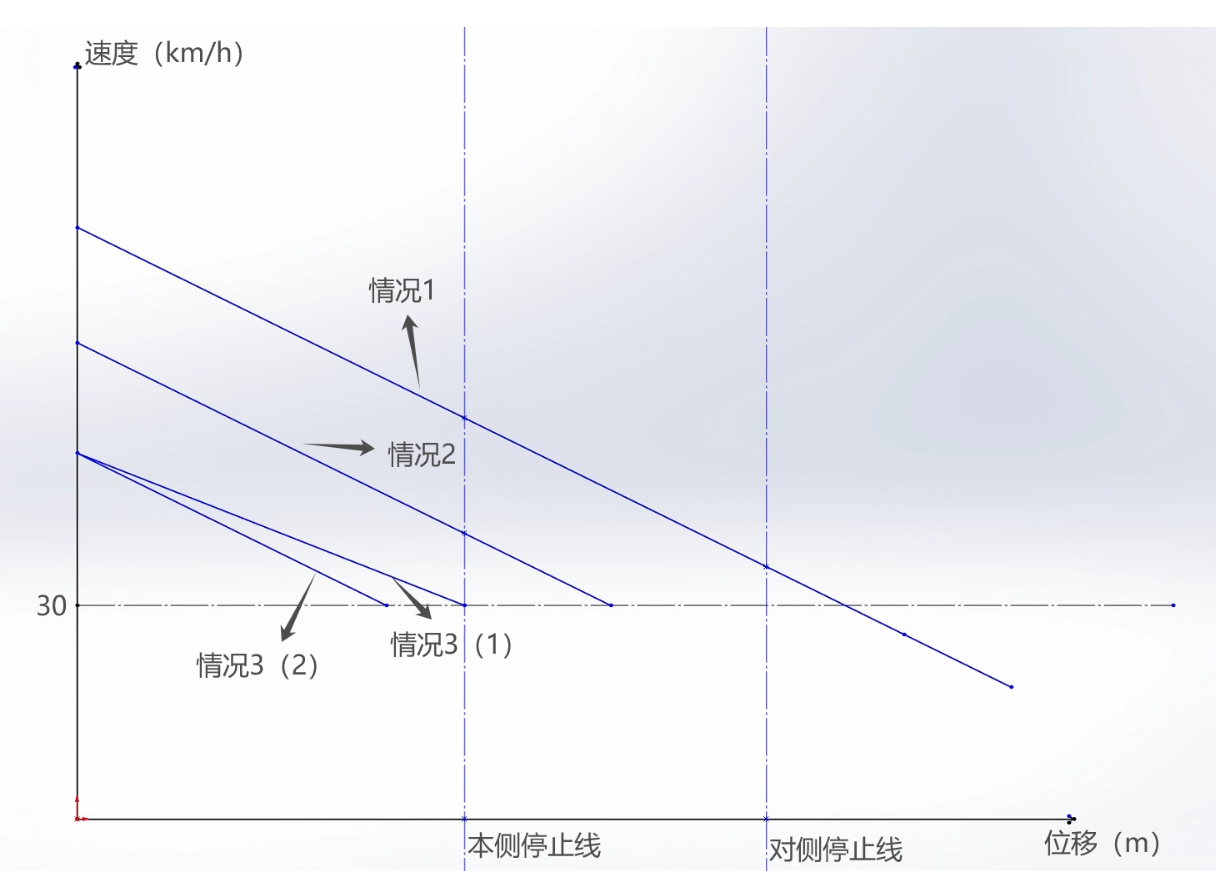
\includegraphics[width=0.7\textwidth]{pics/process}
	\caption{模型二分类示意图}
	\label{fig:proc}
\end{figure}
由于后两种情况中,驾驶员能够在汽车抵达停止线之前成功将车辆停稳,因此接下来的分析将仅针对前三种情形进行深入探讨。

\begin{enumerate}
\item 情况一:汽车全程以$a_1$进行匀减速
	\begin{align*}
		\begin{cases}
				v_{end}^2 - v_0^2 = 2a_1x \\
				x = S + L + H -v_0t_0 \\
				v_{end} - v_0 = a_1t_1
			\end{cases}
	\end{align*}
	即
		$$T= \frac{{\sqrt{v_0^2 + 2a_1(S + L + H - v_0t_0)}-v_0}}{a_1} + t_0$$
\item 情况二:汽车全程先以$a_1$进行匀减速,再以30$km/h$匀速通过路口
	\begin{align*}
	\begin{cases}
		t_1 = \frac{v_F-v_0}{a_1} \\
		s + x_1 - v_0t_0 = \frac{v_F^2 - v_0^2}{2a_1} \\
		x_2 = H + L - x_1\\
		x_2 = t_2v_F
	\end{cases}
	\end{align*}
即
$$T= \frac{v_F - v_0}{a_1} + \frac{H + L - \frac{v_F^2 - v_0^2}{2a_1} - v_0t_0 + S}{v_F} + t_0$$
\item 情况三(1):汽车在到达停止线时刹至30$km/h$,剩余路程匀速
\begin{align*}
	\begin{cases}
		a_2 = \frac{v_F^2 - v_0^2}{2(S-v_0t_0)}\\
		a_2t_1 = v_F - v_0\\
		t_2v_F = H + L
	\end{cases}
\end{align*}
即
$$T= \frac{2(S - v_0t_0)}{v_F + v_0} + \frac{H + L}{v_F} + t_0$$
\item 情况三(2):汽车在到达停止线前刹至30$km/h$,剩余路程匀速
\begin{align*}
	\begin{cases}
		a_1t_1 = v_F - v_0\\
		2a_1x_1 = v_F^2 - v_0^2 \\
		v_Ft_2 = H + L + S - \frac{v_F^2 - v_0^2}{2a_1}-v_0t_0
	\end{cases}
\end{align*}
即
$$T= \frac{v_F - v_0}{a_1} + \frac{H + L + S - \frac{v_F^2 - v_0^2}{2a_1}-v_0t_0}{v_F} + t_0 $$
\end{enumerate}
\subsection{问题二的求解}
为进行黄灯合理时长的确定,需要探究司机的反应感知时间($t_0$)和最大减速度($a_1$),其中,反应感知时间的确定需要数据的收集以确定其对应函数模型,其影响因素主要为初速度和黄灯是否有倒计时。
\subsubsection{数值选取与分析}
考虑在某些特定区域存在在黄灯转红灯有倒计时情况,探究有无倒计时对汽车安全通过时间,即最优黄灯亮灯时长的影响。有倒计时情况下,驾驶员看见倒计时即以更大加速度开始减速,加速度的选取尤为重要。
\begin{itemize}
	\item $a_1$ 和 $t_0$的选取
	\begin{itemize}
		\item 根据\cite{ref1},在无读秒条件下,通过拟合,感知反应时间与速度之间的拟合结果为表\ref{fig:down1},指数函数较其他备选函数,能更好地模拟倒计时条件下最大减速度与黄灯启亮时速度之间的变化关系,公式为:
		$$a_1 = -exp(2340-\frac{52.329}{3.6v_0})$$
		\item 在有读秒条件下,感知反应时间与速度之间的拟合结果为表\ref{fig:down2},对数函数较其他备选函数,能更好地模拟倒计时条件下最大减速度与黄灯启亮时速度之间的变化关系,公式为:
		$$a_1 = 0.045v_0^{1.087}$$
		\item 在无读秒条件下,感知反应时间与速度之间的拟合结果为表\ref{fig:down3},指数函数为最合适的函数模型,公式如下:
		$$t_0 = 2.5exp(-0.018)*3.6v_0$$ 
		\item 在有读秒条件下,感知反应时间与速度之间的拟合结果为表\ref{fig:down4},对数函数为最合适的函数模型,公式为:
		$$t_0 = -1.926\ ln(3.6v_0)+8.703$$
	\end{itemize}
		\begin{figure}[htbp!]
		\centering
		\begin{subfigure}[t]{0.47\textwidth}
			\centering
			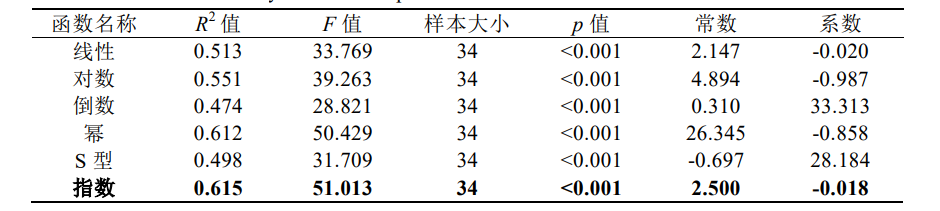
\includegraphics[width=\textwidth]{pics/fyc1}
			\subcaption{无倒计时条件下最小感知反应时间与黄灯启亮时速度之间关系的拟合结果}
			\label{fig:down1}
		\end{subfigure}
		\hfill % 插入空格以分隔两个子图
		\begin{subfigure}[t]{0.47\textwidth}
			\centering
			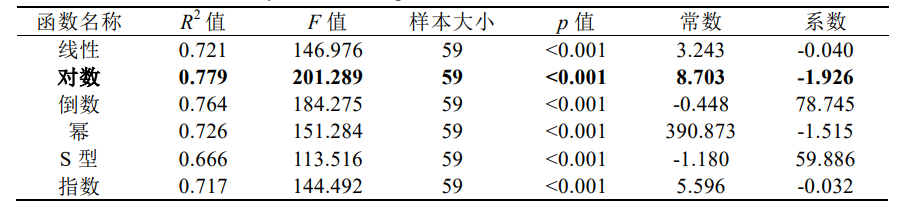
\includegraphics[width=\textwidth]{pics/fyc2}
			\subcaption{有倒计时条件下最小感知反应时间与黄灯启亮时速度之间关系的拟合结果}
			\label{fig:down2}
		\end{subfigure}
		
		\bigskip % 插入额外的空行以分隔两行子图
		\begin{subfigure}[t]{0.47\textwidth}
			\centering
			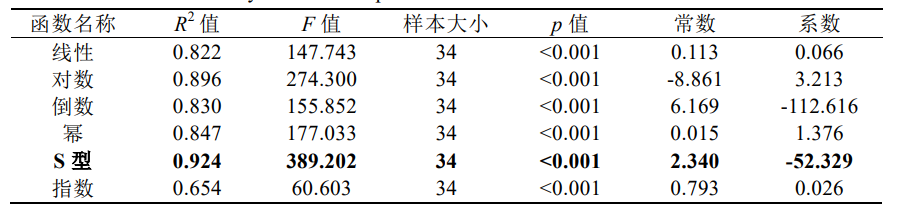
\includegraphics[width=\textwidth]{pics/fyc3}
			\subcaption{无倒计时条件下最大减速度与黄灯启亮时速度之间关系的拟合结果}
			\label{fig:down3}
		\end{subfigure}
		\hfill % 插入空格以分隔两个子图
		\begin{subfigure}[t]{0.47\textwidth}
			\centering
			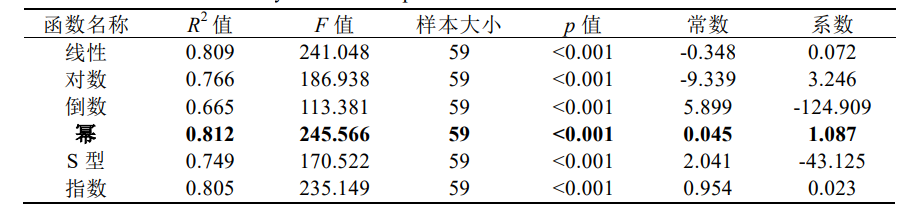
\includegraphics[width=\textwidth]{pics/fyc4}
			\subcaption{有倒计时条件下最大减速度与黄灯启亮时速度之间关系的拟合结果}
			\label{fig:down4}
		\end{subfigure}
		\caption{有无倒计时情况下参数函数拟合结果}
		\label{fig:ref}
	\end{figure}

\end{itemize}


\begin{table}[htbp!]
	\centering
	\begin{tabular}{| c | c | c |} % 定义了三列,每列居中对齐
		\hline
		& \large 有倒计时 & \large 无倒计时 \\ % 表头
		\hline
		\large$a_1(v_0)$ &\large $a_1 = 0.045v_0^{1.087}$ & \large$a_1 = -exp(2340-\frac{52.329}{3.6v_0})$ \\
		\hline
		\large$t_0(v_0)$ & \large$t_0 = -1.926\ ln(3.6v_0)+8.703$ & \large$t_0 = 2.5exp(-0.018)*3.6v_0$ \\
		\hline
	\end{tabular}
	\caption{参考数据公式汇总}
	\label{tab:3x3-table}
\end{table}
\begin{table}[h]
	\centering
	\begin{tabular}{m{5cm}ccc}
		\toprule
		 & \multicolumn{3}{c}{限速值 (km/h)} \\
		\cmidrule{2-4}
		& 无道路中心线 & 同方向单车道& 同方向多车道\\
		\midrule
		城市道路 & 30 & 50 & 70\\
		公路 & 40 & 70& 80\\
		\bottomrule
	\end{tabular}
	\caption{中国城市道路类型及其限速值}
	\label{tab:speed_limits}
\end{table}
\subsubsection{模型一的求解}
根据数值选取中一般情况,取$v_0 = 15m/s, S = 10m, L=4m, H=30m$ ,得到$$T = \frac{S + L + H}{v_0} \approx 3s$$	

结果约等于现有常见的黄灯时长,利用模型二进一步探究各个因素对黄灯时长的具体影响。
\subsubsection{模型二的求解}
\begin{itemize}
	\item $S$范围的选取
	根据文献\cite{ref2}的调研结果,研究发现,无论在信号灯黄灯阶段结束前的倒计时显示与否,当车辆距离交叉路口的距离$S<20m$,几乎所有驾驶员倾向于继续行驶而不采取停车措施。相对地,当距离$S>60m$时,绝大多数驾驶员则选择开始减速并准备停车。基于此,黄灯时长参数的取值范围应为$20m -60m$,更准确地模拟驾驶员在不同距离下的决策行为,在此基础上探究有无黄灯结束倒计时,变量$S$和变量$v_0$对黄灯合理时间$T$的影响。根据图\ref{fig:downt1},$20-40m$为司机犹豫和决策的主要区域,因此本研究最终选取$20-40m$作为$S$取值范围。
\end{itemize}
\begin{figure}[htbp!]
	\centering
	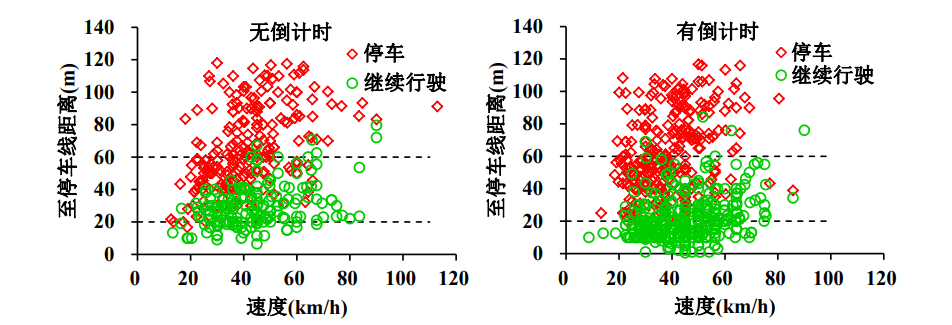
\includegraphics[width=\textwidth]{pics/chooses}
	\caption{在无倒计时(左图)和有倒计时(右图)条件下驾驶行为\cite{ref1}}
	\label{fig:downt1}
\end{figure}
\begin{enumerate}
	\normalsize
	\item 有无黄灯结束倒计时对汽车安全通过时间$T$的影响
	\begin{itemize}
		\item 在固定安全时间
		S的条件下,如图\ref{fig:T1}所示,随着初始速度$v_0$的增加,所需黄灯时间$T$呈现减少的趋势。特别地,在无黄灯倒计时的的情况下,当初始速度为取值区间最小值$v_0=15m/s$,对应的黄灯时间$T$相对较大。同时,在无倒计时情况下当其他变量保持不变,随着初始速度的增加,合理设置的黄灯时间$T$下降速率更为显著。固定$S$,如\ref{fig:T1}所示,随$v_0$增加$T$减小,当变量相同,在有倒计时情况下,随$v_0$增大所需合理黄灯时间$T$下降更快。
		\item 固定$v_0$,如图\ref{fig:T3},随距离$S$的逐渐增加,所需黄灯时间$T$呈现增加的趋势。在无黄灯倒计时的的情况下,当初始速度为取值区间最小值$v_0=15m/s$,对应的黄灯时间$T$相对较大。同时,在无倒计时情况下当其他变量保持不变,随着距离$S$的增加,合理设置的黄灯时间$T$上升更为显著。
	\end{itemize}
	\begin{figure}[htbp!]
		\centering
		\begin{subfigure}[t]{0.45\textwidth}
			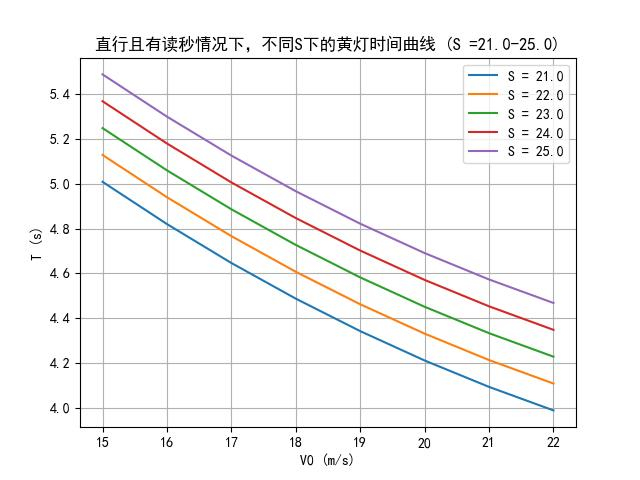
\includegraphics[width=\textwidth]{pics/Time_Curve_S_WCT_STR25.00}
			\subcaption{$S \in [21, 25]$, 有倒计时}
			\label{fig:S25_WCT}
		\end{subfigure}
		\hfill
		\begin{subfigure}[t]{0.45\textwidth}
			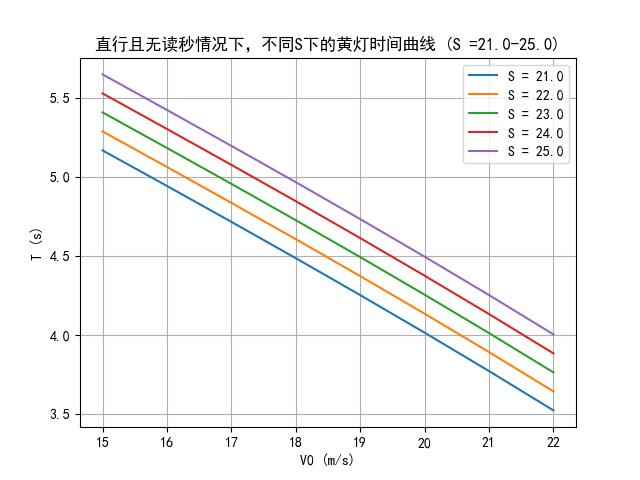
\includegraphics[width=\textwidth]{pics/Time_Curve_S_WOCT_STR25.00}
			\subcaption{$S \in [21, 25]$, 无倒计时}
			\label{fig:S25_WOCT}
		\end{subfigure}
		\\
		\begin{subfigure}[t]{0.45\textwidth}
			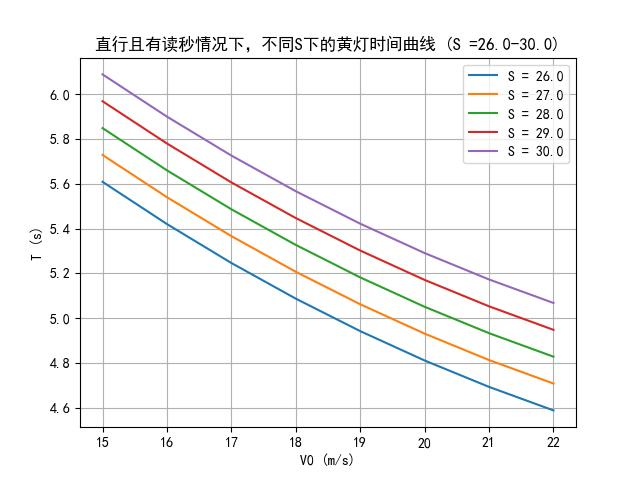
\includegraphics[width=\textwidth]{pics/Time_Curve_S_WCT_STR30.00}
			\subcaption{$S \in [26, 30]$, 有倒计时}
			\label{fig:S30_WCT}
		\end{subfigure}
		\hfill
		\begin{subfigure}[t]{0.45\textwidth}
			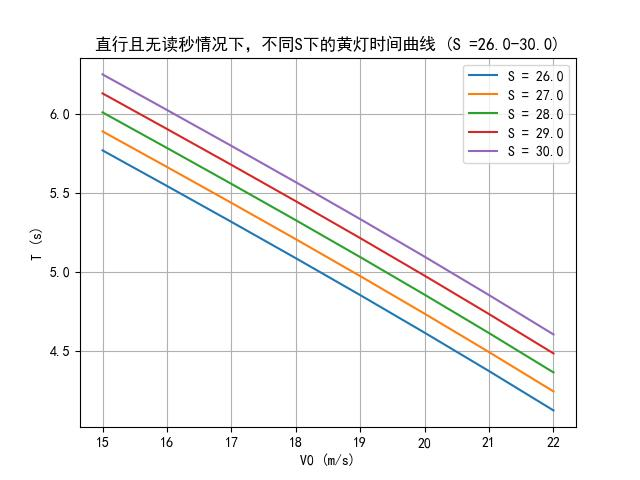
\includegraphics[width=\textwidth]{pics/Time_Curve_S_WOCT_STR30.00}
			\subcaption{$S \in [26, 30]$, 无倒计时}
			\label{fig:S30_WOCT}
		\end{subfigure}
		\caption{不同$S$值下的时间曲线比较(1)}
		\label{fig:T1}
	\end{figure}
	
	
	\item $S$对于汽车安全通过时间$T$的影响
	\begin{itemize}
		\item 当$S$固定,图像\ref{fig:T1}和\ref{fig:T2}显示了在不同绿灯变黄灯时距停止线距离$S$数值下合理黄灯时间$T$随$v_0$变化的曲线,$S$的取值范围为$[21, 40]$(单位为$m$)。随着初速度的增加,曲线呈现下降趋势且斜率随之减小。这意味着在给定$S$的条件下,速度越快,完成整个过程所需的时间越少。
		\item 	当$v_0$固定,图像\ref{fig:T3}显示了在不同$v_0$下合理黄灯时间$T$随$v_0$变化的曲线,$S$的取值范围为$21m-30m$。随着$S$的增加,合理黄灯时长$T$曲线整体增加。
	\end{itemize}
	\begin{figure}[htbp]
		\centering
		\begin{subfigure}[t]{0.45\textwidth}
			\centering
			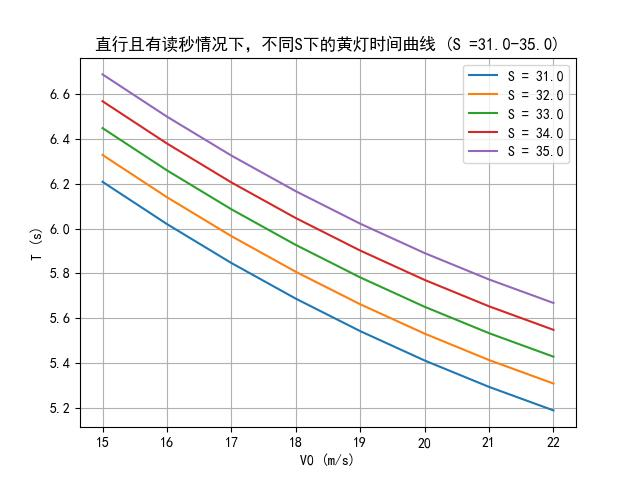
\includegraphics[width=\textwidth]{pics/Time_Curve_S_WCT_STR35.00}
			\subcaption{$S \in [31, 35]$, 有倒计时}
			\label{fig:S35_WCT}
		\end{subfigure}
		\hfill % 插入空格以分隔两个子图
		\begin{subfigure}[t]{0.45\textwidth}
			\centering
			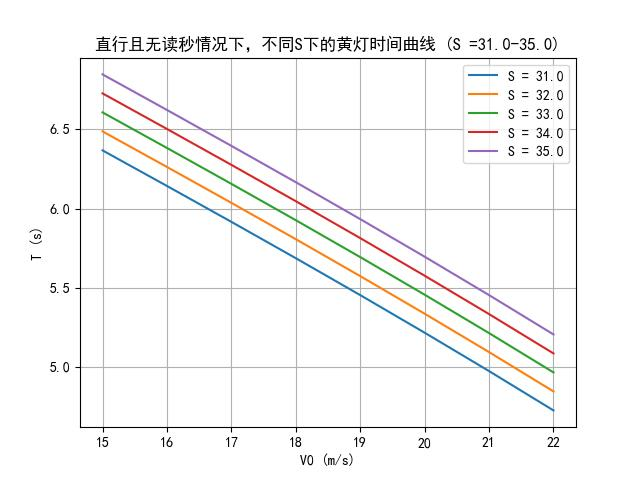
\includegraphics[width=\textwidth]{pics/Time_Curve_S_WOCT_STR35.00}
			\subcaption{$S \in [31, 35]$, 无倒计时}
			\label{fig:S35_WOCT}
		\end{subfigure}
		
		\bigskip % 插入额外的空行以分隔两行子图
		\begin{subfigure}[t]{0.45\textwidth}
			\centering
			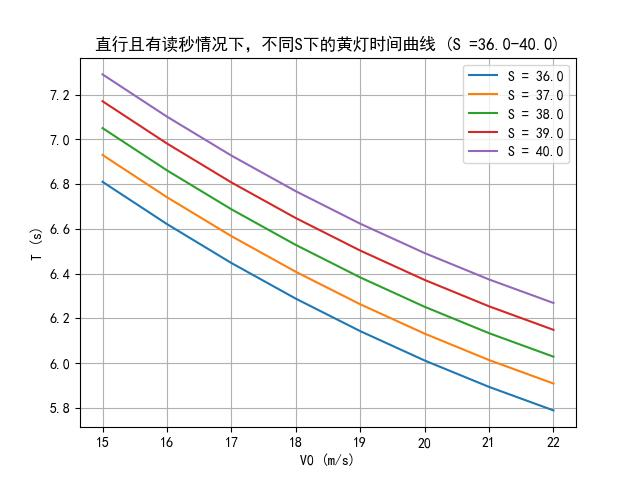
\includegraphics[width=\textwidth]{pics/Time_Curve_S_WCT_STR40.00}
			\subcaption{$S \in [36, 40]$, 有倒计时}
			\label{fig:S40_WCT}
		\end{subfigure}
		\hfill % 插入空格以分隔两个子图
		\begin{subfigure}[t]{0.45\textwidth}
			\centering
			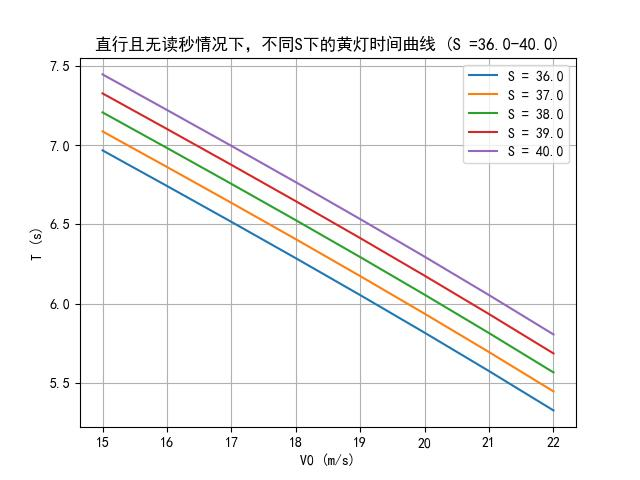
\includegraphics[width=\textwidth]{pics/Time_Curve_S_WOCT_STR40.00}
			\subcaption{$S = \in [36, 40]$, 无倒计时}
			\label{fig:S40_WOCT}
		\end{subfigure}
		\caption{不同安全时间\( S \)值下的时间曲线比较(2)}
		\label{fig:T2}
	\end{figure}
	
	\item $v_0$对于汽车安全通过时间$T$的影响
	\begin{itemize}
		\item 当$S$固定,图像\ref{fig:T2}显示了在不同$S$下合理黄灯时间$T$随$v_0$变化的曲线,$v_0$的取值范围为$15m/s-22m/s$,即$54 km/h-79.2km/h$。随着初速度的增加,曲线呈现下降趋势且斜率随之减小。这意味着在给定$S$的条件下,速度越快,完成整个过程所需的时间越少。
		\item 	当$v_0$固定,图像\ref{fig:T3}显示了在不同$v_0$下合理黄灯时间$T$随$v_0$变化的曲线,$S$的取值范围为$21m-30m$。随着$S$的增加,合理黄灯时长$T$曲线整体增加,且$v_0$越小,$T$增加越快。
	\end{itemize}
	\begin{figure}[htbp!]
		\centering
		\begin{subfigure}[t]{0.45\textwidth}
			\centering
			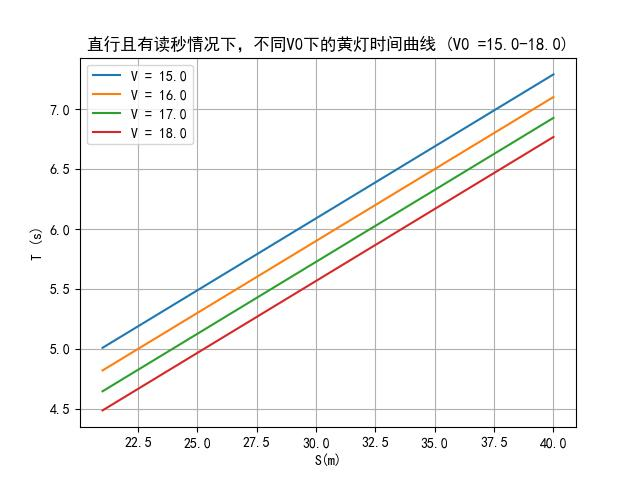
\includegraphics[width=\textwidth]{pics/Time_Curve_V0_WCT_STR18.0}
			\subcaption{$v_0 \in [15,18]$, 无倒计时}
			\label{fig:v01}
		\end{subfigure}
		\hfill
		\begin{subfigure}[t]{0.45\textwidth}
			\centering
			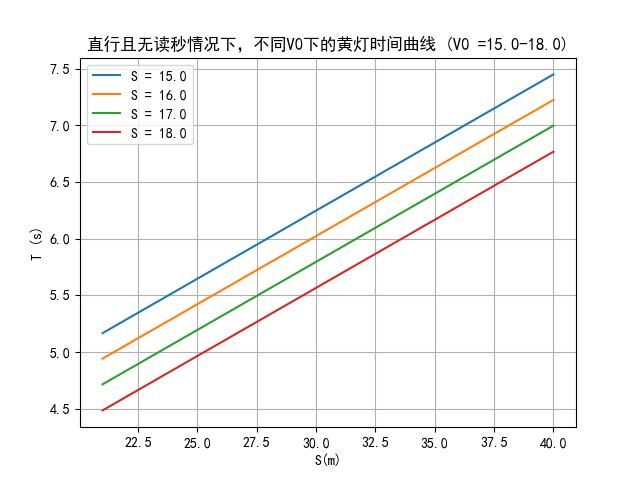
\includegraphics[width=\textwidth]{pics/Time_Curve_V0_WOCT_STR18.0}
			\subcaption{$v_0 \in [15,18]$, 无倒计时}
			\label{fig:v02}
		\end{subfigure}
		\\
		\begin{subfigure}[t]{0.45\textwidth}
			\centering
			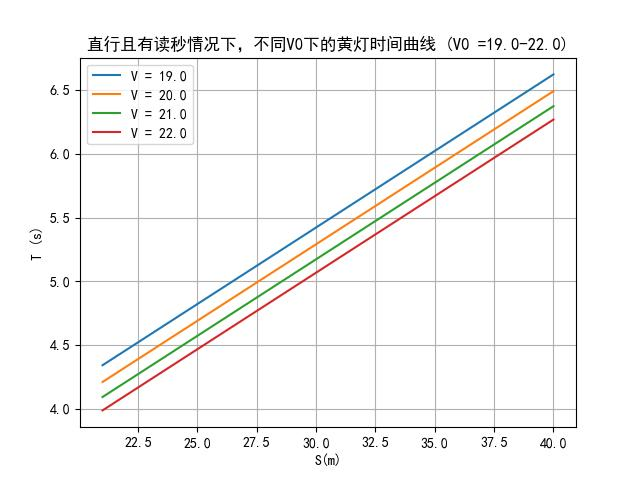
\includegraphics[width=\textwidth]{pics/Time_Curve_V0_WCT_STR22.0}
			\subcaption{$v_0 \in [19,22]$$S = 40$, 无倒计时}
			\label{fig:v03}
		\end{subfigure}
		\hfill
		\begin{subfigure}[t]{0.45\textwidth}
			\centering
			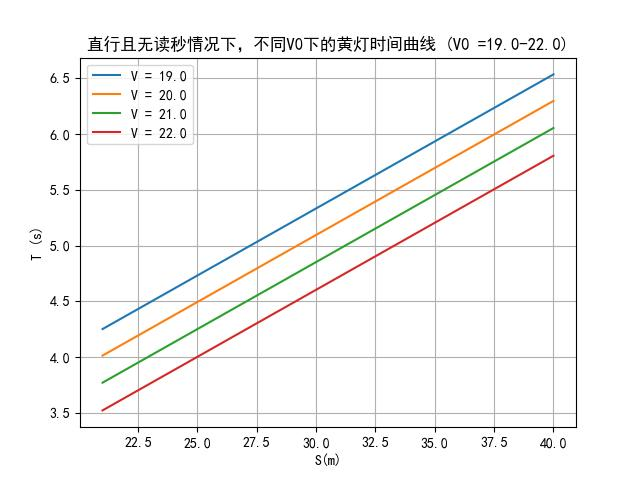
\includegraphics[width=\textwidth]{pics/A} % 注意这里文件名需要与原始图像对应
			\subcaption{$v_0 \in [19,22]$, 无倒计时}
			\label{fig:v04}
		\end{subfigure}
		\caption{不同初始速度和安全时间下的时间曲线比较}
		\label{fig:T3}
	\end{figure}
	\begin{figure}[htbp!]
		\centering
		\begin{tikzpicture} [>=latex, scale = 0.5]
			% 画半圆,中心在(0,0),半径为2cm
			\draw (-3,2) arc (270:360:1cm);
			\draw (-2,-3) arc (0:90:1cm);
			\draw (2,3) arc (180:270:1cm);
			\draw (3,-2) arc (90:180:1cm);
			% 可以添加一些辅助线或标记
			\fill (0,0) circle (2pt); % 标记圆心
			\draw (3,2) -- (7,2); 
			\draw (3,-2) -- (7,-2); 
			\draw (-3,2) -- (-7,2); 
			\draw (-3,-2) -- (-7,-2); 
			\draw (2,3) -- (2,7); 
			\draw (2,-3) -- (2,-7); 
			\draw (-2,-3) -- (-2,-7); 
			\draw (-2,3) -- (-2,7); 
			\draw (-1,0) -- (1,0); % x轴
			\draw (0,-1) -- (0,1); % y轴
			\draw (0,3) -- (0,7); 
			\draw (0,-3) -- (0,-7); 
			\draw (3,0) -- (7,0); 
			\draw (-3,0) -- (-7,0); 
			\draw[line width=1.5pt, ->] (1,-4) -- (1,-2.2);
			\draw[line width=1.5pt] (5/3,-4) -- (5/3,-2.7);
			\draw[line width=1.5pt, ->] (5/3,-2.7) -- (2,-2.2);
			\draw[line width=1.5pt] (1/3,-4) -- (1/3,-2.7);
			\coordinate (A) at (1/3,-2);
			\draw[blue, dashed, line width=0.8pt] (A) arc (0:90:2.33cm);
			\draw[blue, dashed, line width=0.8pt] (1/3,-2) -- (1/3,-2.7);
			\draw[blue, dashed, line width=0.8pt] (-2,1/3) -- (-2.7,1/3);
			\draw[blue, dashed, line width=0.8pt] (-2,1/3) -- (-2,-2);
			\draw[blue, dashed, line width=0.8pt] (1/3,-2) -- (-2,-2);
			\node[left] at (-2,-1) {$r = \frac{7}{6} H$};
			\node[above] at (1, -0.5) {$l = \frac{7}{24}\pi H$};
			\draw[ ->] (-2,2.5) -- (-0.5,2.5);
			\node[right] at (-0.5,2.5) {$H$};
			\draw[ ->] (2,2.5) -- (0.5,2.5);
		\end{tikzpicture}
		\caption{左转道与直行道路口经过距离$H$}
		\label{left}
	\end{figure}
		\item 不同车道对于汽车安全通过时间$T$的影响
	\begin{itemize}
		\item 如图\ref{left}所示,在路口宽度为$H$情况下左转车道正常车辆行驶距离约为$\frac{7}{24}\pi H$, 将其带入模型二,分别比较在固定$S$和$v_0$时直行和左转时合理黄灯时长$T$的不同。
		\item 	图像\ref{fig:str1}和\ref{fig:turn1}显示了在不同$S$下合理黄灯时间$T$随$v_0$变化的曲线,	图像\ref{fig:str2}和\ref{fig:Turn2}显示了在不同$v_0$下合理黄灯时间$T$随$S$变化的曲线,观察图像可以发现,直行需要的黄灯时长普遍高于相同情况下左转所需时长,在现实生活运用中可以据此为左转道和直行道设置不同的黄灯长度,节省时间成本提高效率。
	\end{itemize}
\end{enumerate}
	\begin{figure}[htbp!]
	\centering
	\begin{subfigure}[t]{0.45\textwidth}
		\centering
		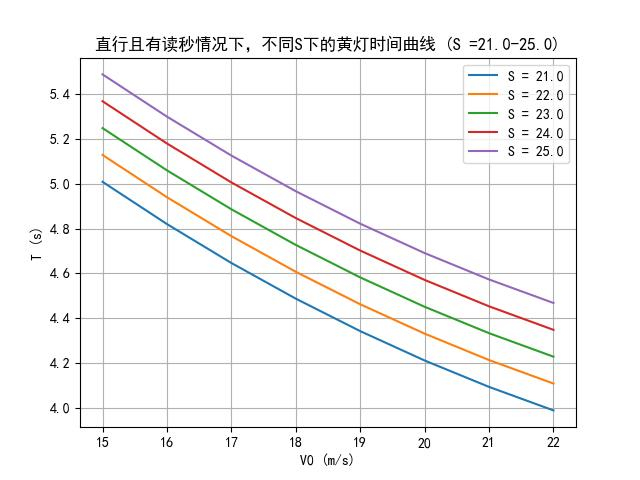
\includegraphics[width=\textwidth]{pics/Time_Curve_S_WCT_STR25.00}
		\subcaption{$S$固定, 直行有倒计时}
		\label{fig:str1}
	\end{subfigure}
	\hfill
	\begin{subfigure}[t]{0.45\textwidth}
		\centering
		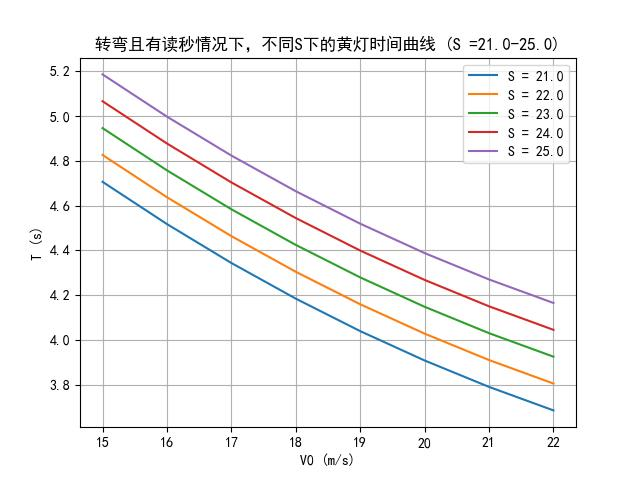
\includegraphics[width=\textwidth]{pics/Time_Curve_S_WCT_Turn25.00}
		\subcaption{$S$固定, 左转有倒计时}
		\label{fig:turn1}
	\end{subfigure}
	\\
	\begin{subfigure}[t]{0.45\textwidth}
		\centering
		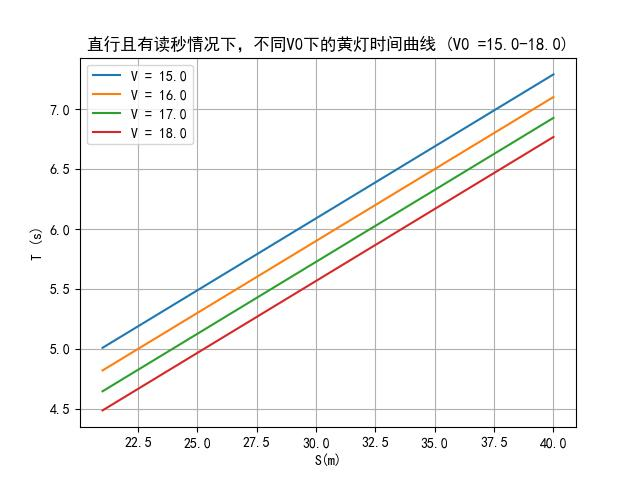
\includegraphics[width=\textwidth]{pics/Time_Curve_V0_WCT_STR18.0}
		\subcaption{$v_0$固定, 直行有倒计时}
		\label{fig:str2}
	\end{subfigure}
	\hfill
	\begin{subfigure}[t]{0.45\textwidth}
		\centering
		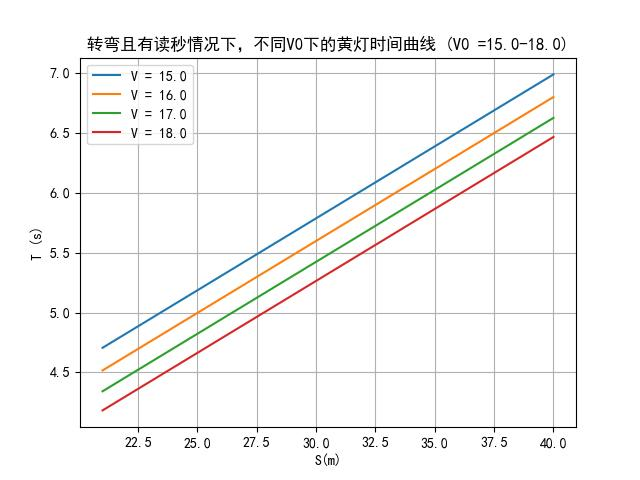
\includegraphics[width=\textwidth]{pics/Time_Curve_V0_WCT_Turn18.0} % 注意这里文件名需要与原始图像对应
		\subcaption{$v_0$固定, 左转有倒计时}
		\label{fig:Turn2}
	\end{subfigure}
	\caption{不同方向下的合理黄灯时间曲线比较}
	\label{fig:T5}
\end{figure}


\subsection{问题三的求解}
\normalsize
问题二解得的合理黄灯时长(得出的黄灯时长主要由末行车的行驶时间决定)大致在6-7$s$,高于现行得到一般标准3-4$s$,大致原因如下:
\begin{enumerate}
	\item 如表\ref{tab:yellow_light_duration},在现行黄灯执行标准$3-4s$内,大部分车辆都能安全通过本侧停止线,进入交叉路口,但仅有少部分车辆(当黄灯时长为$3s$时甚至没有车能通过交叉路口)能通过对侧停止线,大部分车辆在黄灯转红时依然逗留在交叉路口内,安全隐患较大。但当将标准提高至上述模型计算值时,基本所有车辆都能安全通过交叉路口。
	\item 在计算中考虑了为了严格遵守交规所进行的适当减速,因此会增加末行车的总体行驶时间,从而造成合理黄灯时间$T$的增加
	\item 在计算中考虑了防止碰撞行人和前方减速车辆等突发情况而进行的适当减速,一定在程度上也增加了合理黄灯时间
	\item 在计算中考虑了每辆车的车身长度,使末行车行驶时间变长
\end{enumerate}
黄灯市场较长带来的潜在优势有:
\begin{itemize}
	\item 提供充分的反应时间:延长的黄灯时长为驾驶员提供了额外的决策时间,尤其在交通高峰或不利天气条件下显得尤为重要。
	\item 减少急刹车情况:充足的黄灯时长允许驾驶员有更多的时间来做出反应,从而可能降低因紧急制动而导致的交通事故发生概率。
	\item 增强道路利用率和流畅性:较长的黄灯时长有助于更多车辆在信号灯变换前通过路口,有助于缓解交通拥堵,提高道路使用率和效率。
\end{itemize}

黄灯时长较长也存在一些潜在的缺点:
\begin{itemize}
	\item 增加通行时间的不确定性:过长的黄灯时长可能使驾驶员难以准确决策是否、何时应加速通过路口,这种不确定性可能对交通反而产生负面影响。
	\item 对路口容量的影响:在交通密集区域,较长的黄灯时长可能导致路口通行能力降低,从而引发交通拥堵和延误。
	\item “冒险主义者”:黄灯时长的延长可能诱使部分驾驶员在黄灯期间冒险通过,反而增强了违规的风险。
	\item 在当前的研究中,尚未计入两侧车道交通信号灯由红色转为绿色时车辆的起步时间以及驾驶员的反应时间。这一忽略可能一定程度上导致计算所得的合理黄灯时长结果偏高,从而造成时间资源的浪费。
\end{itemize}

\begin{table}[ht]
	\centering % 表格居中
	\begin{tabular}{| c | c | c |} % 创建四列
		\hline % 上边框线
		黄灯时长(s) & 通过停止线车辆百分比(\%) & 对侧停止线百分比(\%) \\
		3 & 88.44\% & 0.00\% \\
		4 & 100.00\% & 2.19\%  \\
		5 & 100.00\% & 27.81\%  \\
		6 & 100.00\% & 67.81\%  \\
		7 & 100.00\% & 96.88\%  \\
		8 & 100.00\% & 100.00\%  \\
		\bottomrule % 下边框线
	\end{tabular}
	\caption{黄灯时长与通过停止线车辆百分比的关系} % 表格标题
	\label{tab:yellow_light_duration} % 表格标签
\end{table}
%\begin{table}[htbp!]
%	\centering
%	\begin{tabular}{| c | c | c |} % 定义了三列,每列居中对齐
%		\hline
%		& \large 有倒计时 & \large 无倒计时 \\ % 表头
%		\hline
%		\large$a_1(v_0)$ &\large $a_1 = 0.045v_0^{1.087}$ & \large$a_1 = -exp(2340-\frac{52.329}{3.6v_0})$ \\
%		\hline
%		\large$t_0(v_0)$ & \large$t_0 = -1.926\ ln(3.6v_0)+8.703$ & \large$t_0 = 2.5exp(-0.018)*3.6v_0$ \\
%		\hline
%	\end{tabular}
%	\caption{数据公式汇总}
%	\label{tab:3x3-table}
%\end{table}





%\subsection{龙格库塔法简介}
%龙格库塔法\cite{ref5}是一类解微分方程的数值算法, 其中较常见的是四阶龙格库塔法,其精度较高,这里不进行推导,仅仅给出公式:
%\begin{align*}
%	\begin{cases}
%		y_{k+1} = y_k + \dfrac{h}{6}(k_1+2k_2+2k_3+k_4) \\
%		k_{1} = f(t_k,y_k)\\
%		k_{2} = f(t_k+\frac{h}{2},y_k+\frac{h}{2}k_1)\\
%		k_{3} = f(t_k+\frac{h}{2},y_k+\frac{h}{2}k_2)\\
%		k_{4} = f(t_k+h,y_k+k_3)
%	\end{cases}
%\end{align*}
%之后我们将微分方程组带入MATLAB并利用四阶龙格库塔古典模型求解。
\section{模型的评价,改进与推广}
\subsection{模型的评价}
\subsubsection{优点}
\begin{itemize}
	\item 该模型设计考虑了广泛的适用性,能够适应多变的交通环境和驾驶员行为。
	\item 模型对不同交通情境进行了细致的分类,并针对每一类别进行了深入的讨论,以确保模型的有效性,通过个性化定制,黄灯时间的设定展现出更高的灵活性,从而优化交通流的控制和提高道路安全。
	\item 在本研究中,所选取的加速度值并非最大理论值,而是在确保行车安全的前提下,经过审慎考量后确定的合理数值,旨在实现在不同交通条件下的最优驾驶行为。
\end{itemize}
\subsubsection{缺点}
\begin{itemize}
	\item 该模型建立在严格遵守交通规则的假设之上,但在现实生活中通常存在着在黄灯的最后几秒驾驶员“冲线”加速的情况,此类情况下加速度为正,需另行考虑。
	\item 模型需要进一步考虑现实的偶发因素,如极端天气,路面情况\cite{ref3}等,这些因素可能对驾驶员的反应时间和初速度产生显著影。
\end{itemize}
\subsection{模型的改进与推广}
\begin{itemize}
	\item 在本次解题中我们未对各影响因子进行相关性分析,在收集到更完备的数据的前提下,我们可以构建聚类模型,将具有相似性质的因素进行归类,求出关于黄灯信号时长$T$更完备的方程
	\item 在有利润方程的前提下,设置一定约束条件,可以采用线性规划模型进行运算得到更准确的结果。
	\item 在现实生活中还有可能存在绿灯变黄灯存在倒计时的情况,需要进一步讨论。
	\end{itemize}



\section{模型的检验}
\subsection{相关性检验}
利用问题三得到数据,我们对模型涉及参数进行相关性检验,皮尔森相关系数热力图结果如图\ref{fig:cos}所示:

研究结果表明,车辆在本侧停止线末尾的通过百分比以及在对侧停止线末尾的通过百分比与黄灯时长之间存在显著的线性相关性。进一步地,通过对车辆通过率(即车辆尾部已完全通过对侧停止线)与黄灯时长进行线性回归分析,我们得到了以下回归方程:$$\text{通过率} = -0.01584821428571414x^2+0.40808035714285573x-1.174017857142853$$

其中,$x$代表黄灯时长。根据该方程可以推断,在当前黄灯时长的基础上,适当延长黄灯时间将有助于提高车辆的通过率。我们可以通过提高黄灯时间提高汽车通过率,提升城市交通车流安全性。
\begin{figure}[htbp!]
		\centering
		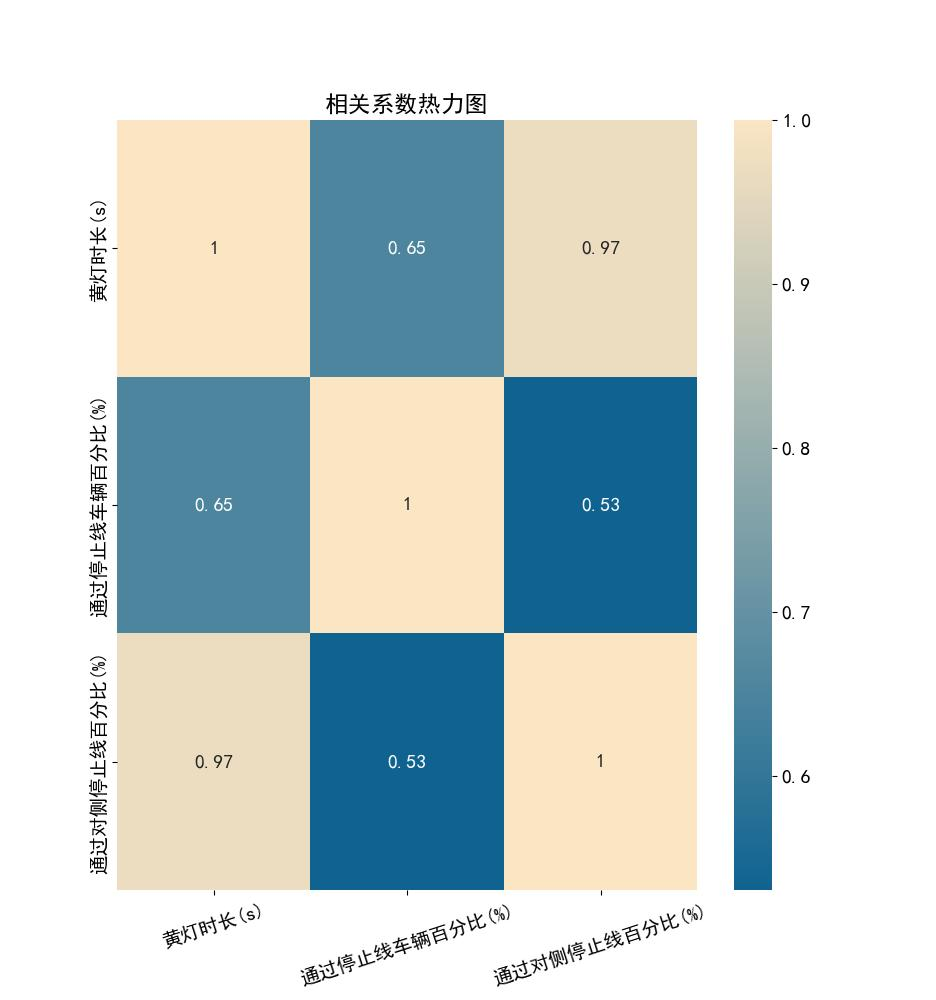
\includegraphics[width=0.5\textwidth]{pics/corres}
		\caption{相关系数热力图矩阵}
		\label{fig:cos}
\end{figure}
\begin{figure}[htbp!]
	\centering
	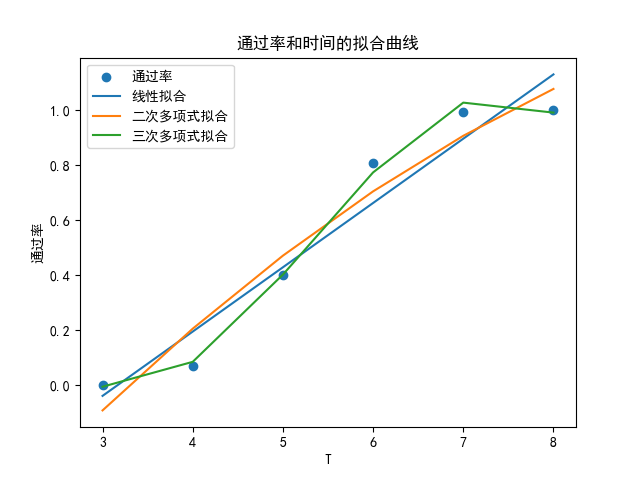
\includegraphics[width=0.5\textwidth]{pics/linear}
	\caption{通过时率与黄灯时间拟合}
	\label{fig:linear}
\end{figure}

\newpage




\begin{thebibliography}{99}  
	\bibitem{ref1}付云川. 信号交叉口黄灯两难区边界建模及风险评估方法研究[A]. 高等教育出版社,2015:12.
	\bibitem{ref2}李克平,杨佩昆,倪颖.城市道路交叉口信号控制中的黄灯问题[J]. 城市交通, 2010, 8(4):67-72
	\bibitem{ref3}焦兴旺,张福生,黄柄胜,赵寅. 基于黄灯困境区的相位安全切换时机研究[J]. 湖南交通科技, 2023, 49(4):184-191.
%	\bibitem{ref4}尼古拉斯·迪方佐. 谣言心理学[A]. 机械工业出版社,2021:8.
%	\bibitem{ref5}房少梅,王霞. 微分方程数值解[A]. 国防工业出版社,2016:5.
\end{thebibliography}
\begin{appendices}
\pagestyle{empty}
\section*{}
\newpage
\textbf{\textcolor[rgb]{0.00,0.00,0.00}{程序一:Python模拟模型二合理黄灯时长:}}
\lstinputlisting[language=Matlab]{./code/Newfunction.py}

\textbf{\textcolor[rgb]{0.00,0.00,0.00}{程序二:程序一对应相关系数热力图:}}
\lstinputlisting[language=Matlab]{./code/Heatmap.py}

%\textbf{\textcolor[rgb]{0.00,0.00,0.00}{程序三:MATLAB模拟不同$\lambda$对谣言传播的影响(模型1):}}
%\lstinputlisting[language=Matlab]{./code/SIR_RK4classic_a.m}
%
%\textbf{\textcolor[rgb]{0.00,0.00,0.00}{程序四:程序三对应微分方程组:}}
%\lstinputlisting[language=Matlab]{./code/ValueRu_a.m}
%
%\textbf{\textcolor[rgb]{0.00,0.00,0.00}{程序五:MATLAB模拟不同$\mu$对谣言传播的影响(模型1):}}
%\lstinputlisting[language=Matlab]{./code/SIR_RK4classic_a.m}
%
%\textbf{\textcolor[rgb]{0.00,0.00,0.00}{程序六:程序五对应微分方程组:}}
%\lstinputlisting[language=Matlab]{./code/ValueRu_a.m}
%
%\textbf{\textcolor[rgb]{0.00,0.00,0.00}{程序七:MATLAB模拟中途$\mu$有改变的情况(模型1):}}
%\lstinputlisting[language=Matlab]{./code/SIR_classic2mu.m}
%
%\textbf{\textcolor[rgb]{0.00,0.00,0.00}{程序八:程序七对应微分方程组1:}}
%\lstinputlisting[language=Matlab]{./code/ValueRu_1.m}
%
%\textbf{\textcolor[rgb]{0.00,0.00,0.00}{程序八:程序七对应微分方程组2:}}
%\lstinputlisting[language=Matlab]{./code/ValueRu_2.m}
%
%\textbf{\textcolor[rgb]{0.00,0.00,0.00}{程序九:MATLAB模拟谣言传播情况(模型2):}}
%\lstinputlisting[language=Matlab]{./code/SIRJW_RK4classic.m}
%
%\textbf{\textcolor[rgb]{0.00,0.00,0.00}{程序十:程序九对应微分方程组:}}
%\lstinputlisting[language=Matlab]{./code/ValueRu5.m}


%\newpage
%\def\thesection{A}
%\renewcommand{\thetable}{\wuhao A-\arabic{table}}
%\setcounter{table}{0}
%\section*{数据表格}
%\textcolor[rgb]{0.98,0.00,0.00}{\textbf{表格数据:}}
%\input{Appendices1}

\end{appendices}
\end{document}